\chapter{Fundamental Algorithms}
\label{chap:fundamental_algorithms}

\begin{figure}[ht]
	\hfill
	\begin{minipage}{0.5\textwidth}
		\centering
		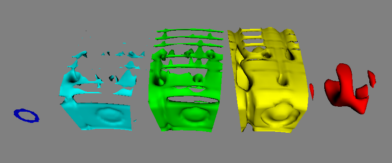
\includegraphics{VTKTextbook-54}\\
		\caption*{\texttt{Isosurfaces of a combustor dataset computed at multiple values..}}
	\end{minipage}
\end{figure}

\firstletter{W}e have seen how to represent basic types of visualization data such as image data, structured grids, unstructured grids, and polygonal data.
This chapter explores methods to transform this data to and from these various representations, eventually generating graphics primitives that we can render.
These methods are called algorithms, and are of special interest to those working in the field of visualization.
Algorithms are the verbs that allow us to express our data in visual form.
By combining these verbs appropriately, we can reduce complex data into simple, readily comprehensible sentences that are the power of data visualization.

\section{Introduction}

The algorithms that transform data are the heart of data visualization.
To describe the various transformations available, we need to categorize algorithms according to the structure and type of transformation.
By structure we mean the effects that transformation has on the topology and geometry of the dataset.
By type we mean the type of dataset that the algorithm operates on.

Structural transformations can be classified in four ways, depending on how they affect the geometry, topology, and attributes of a dataset.

\begin{itemize}

\item \emph{Geometric transformations} alter input geometry but do not changed the topology of the dataset. For example, if we translate, rotate, and/or scale the points of a polygonal dataset, the topology does not change, but the point coordinates, and therefore the geometry, does.

\item \emph{Topological transformations} alter input topology but do not change geometry and attribute data. Converting a dataset type from polygonal data to unstructured grid data, or from image data to unstructured grid, changes the topology but not the geometry. More often, however, the geometry changes whenever the topology does, so topological transformation is uncommon.

\item \emph{Attribute transformations} convert data attributes from one form to another, or create new attributes from the input data. The structure of the dataset remains unaffected. Computing vector magnitude or creating scalars based on elevation are data attribute transformations.

\item \emph{Combined transformations} change both dataset structure and attribute data. For example, computing contour lines or surfaces is a combined transformation.

\end{itemize}

We also may classify algorithms according to the type of data they operate on, or the type of data they generate. By type, we most often mean the type of attribute data, such as scalars or vectors. Typical categories include:

\begin{itemize}

\item \emph{Scalar algorithms} operate on scalar data. For example, the generation of contour lines of temperature on a weather map.

\item \emph{Vector algorithms} operate on vector data. Showing oriented arrows of airflow (direction and magnitude) is an example of vector visualization.

\item \emph{Tensor algorithms} operate on tensor matrices. An example of a tensor algorithm is to show the components of stress or strain in a material using oriented icons.

\item \emph{Modelling algorithms} generate dataset topology or geometry, or surface normals or texture data. Modelling algorithms tend to be the catch-all category for many algorithms, since some do not fit neatly into any single category mentioned above. For example, generating glyphs oriented according to the vector direction and then scaled according to the scalar value, is a combined scalar/vector algorithm. For convenience we classify such an algorithm as a modelling algorithm, because it does not fit squarely into any other category.

\end{itemize}

Algorithms also can be classified according to the type of data they process. This is the most common scheme found in the visualization literature. However, this scheme is not without its problems. Often the categories overlap, resulting in confusion. For example, a category (not mentioned above) is \emph{volume visualization}, which refers to the visualization of volume data (or in our terminology, image data). This category was initially created to describe the visualization of scalar data arranged on a volume, but more recently, vector (and even tensor) data has been visualized on a volume. Hence, we have to qualify our techniques to \emph{volume vector visualization}, or other potentially confusing combinations.

In the text that follows, we will use the attribute type classification scheme: scalar, vector, tensor, and modelling. In cases where the algorithms operate on a particular dataset type, we place them in the appropriate category according to our best judgment. Be forewarned, though, that alternative classification schemes do exist, and may be better suited to describing the true nature of the algorithm.

\begin{figure}[!htb]
	\centering
	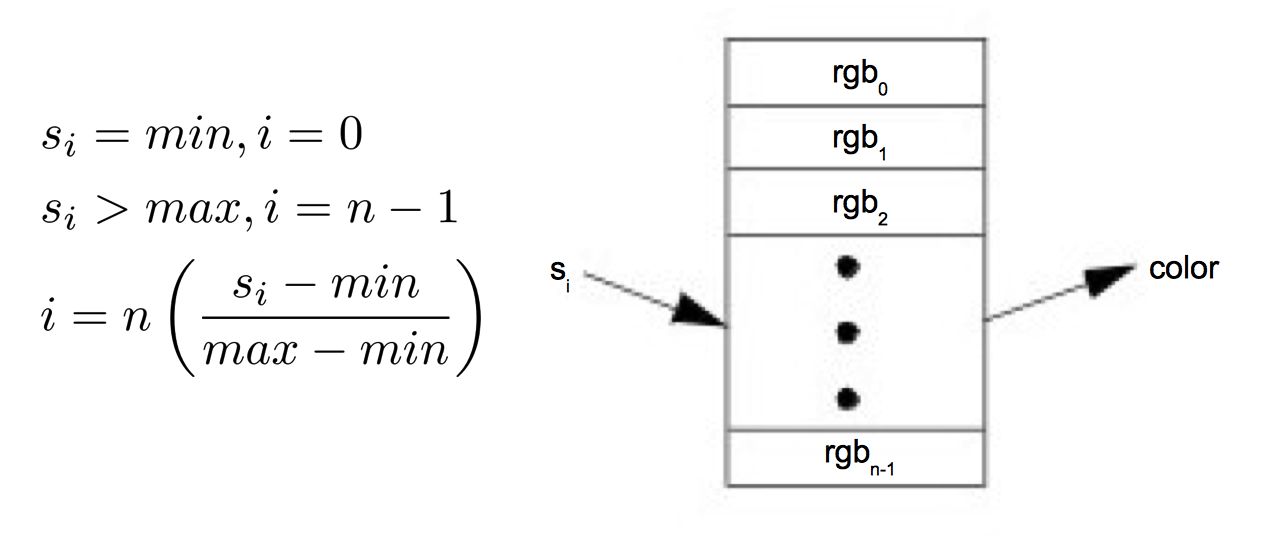
\includegraphics[width=0.8\textwidth]{Figure6-1}\\
	\caption{Mapping scalars to colors via a lookup table.}\label{fig:Figure6-1}
\end{figure}

\section{Generality Versus Efficiency}
Most algorithms can be written specifically for a particular dataset type, or more generally, treating any dataset type. The advantage of a specific algorithm is that it is usually faster than a comparable general algorithm. (See "Other Data Abstractions" on page138 where we discussed the tradeoff between abstract and concrete forms.) An implementation of a specific algorithm also may be more memory efficient and its implementation may better reflect the relationship between the algorithm and the dataset type it operates on.

One example of this is contour surface creation. Algorithms for extracting contour surfaces were originally developed for volume data, mainly for medical applications. The regularity of volumes lends itself to efficient algorithms. However, the specialization of volume-based algorithms precludes their use for more general datasets such as structured or unstructured grids. Although the contour algorithms can be adapted to these other dataset types, they are less efficient than those for volume datasets.

Our presentation of algorithms favors the more general implementations. In some special cases we will describe performance improving techniques for particular dataset types. Refer to the bibliography at the end of each chapter for detailed descriptions of specialized algorithms.

\section{Scalar Algorithms}

Scalars are single data values associated with each point and/or cell of a dataset. (Recall that in the \emph{Visualization Toolkit} we associate data with points.) Because scalar data is commonly found in real-world applications, and because scalar data is so easy to work with, there are many different algorithms to visualize it.

\subsection{Color Mapping}

\emph{Color mapping} is a common scalar visualization technique that maps scalar data to colors, and displays the colors on the computer system. The scalar mapping is implemented by indexing into a \emph{color lookup table}. Scalar values serve as indices into the lookup table.

The mapping proceeds as follows. The lookup table holds an array of colors (e.g., red, green, blue components or other comparable representations). Associated with the table is a minimum and maximum \emph{scalar range (min, max)} into which the scalar values are mapped. Scalar values greater than the maximum range are clamped to the maximum color, scalar values less than the minimum range are clamped to the minimum color value. Then, for each scalar value $x_i$, the index $i$ into the color table with n entries (and 0-offset) is given by \ref{fig:Figure6-1}.

A more general form of the lookup table is called a transfer function. A transfer function is \ref{fig:Figure6-2} maps any expression that maps scalar value into a color specification. For example, scalar values into separate intensity values for the red, green, and blue color components. We can also use transfer functions to map scalar data into other information such as local transparency. (Transfer functions are discussed in more detail in ``Transparency and Alpha Values'' on \pageref{sec:transparency_alpha} and ``Volume Rendering'' on \pageref{sec:volume_rendering}.
\ref{fig:Figure6-2} maps any expression that maps scalar value into a color specification. For example, scalar values into separate intensity values for the red, green, and blue color components.
We can also use transfer functions to map scalar data into other information such as local transparency.
(Transfer functions are discussed in more detail in ``Transparency and Alpha Values`` on page213
and “Volume Rendering” on \pageref{sec:volume_rendering}.)
A lookup table is a discrete sampling of a transfer function.
We can create a lookup table from any transfer function by sampling the transfer function at a set of discrete points.

Color mapping is a one-dimensional visualization technique. It maps one piece of information (i.e., a scalar value) into a color specification. However, the display of color information is not limited to one-dimensional displays. Often we use color information mapped onto 1D, 2D, or 3D objects. This is a simple way to increase the information content of our visualizations.

The key to color mapping for scalar visualization is to choose the lookup table entries carefully. \ref{fig:Figure6-3} shows four different lookup tables used to visualize gas density as fluid flows through a combustion chamber. The first lookup table is gray-scale. Grayscale tables often provide better structural detail to the eye. The other three images in \ref{fig:Figure6-3} use different color lookup tables. The second uses rainbow hues from blue to red. The third uses rainbow hues arranged from red to blue. The last table uses a table designed to enhance contrast. Careful use of colors can often enhance important features of a dataset. However, any type of lookup table can exaggerate unimportant details or create visual artifacts because of unforeseen interactions between data, color choice, and human physiology.

Designing lookup tables is as much art as it is science. From a practical point of view, tables should accentuate important features, while minimizing less important or extraneous details. It is also desirable to use palettes that inherently contain scaling information. For example, a color rainbow scale from blue to red is often used to represent temperature scale, since many people associate "blue" with cold temperatures, and "red" with hot temperatures. However, even this scale is problematic: a physicist would say that blue is hotter than red, since hotter objects emit more blue light (i.e., shorter wavelength) than red. Also, there is no need to limit ourselves to "linear" lookup tables. Even though the mapping of scalars into colors has been presented as a linear operation (\ref{fig:Figure6-1}, the table itself need not be linear. That is, tables can be designed to enhance small variations in scalar value using logarithmic or other schemes, improving the comfort level and engaging the human observer more deeply in the presentation of data improves the effectiveness of communication.

\begin{figure}[!htb]
	\centering
	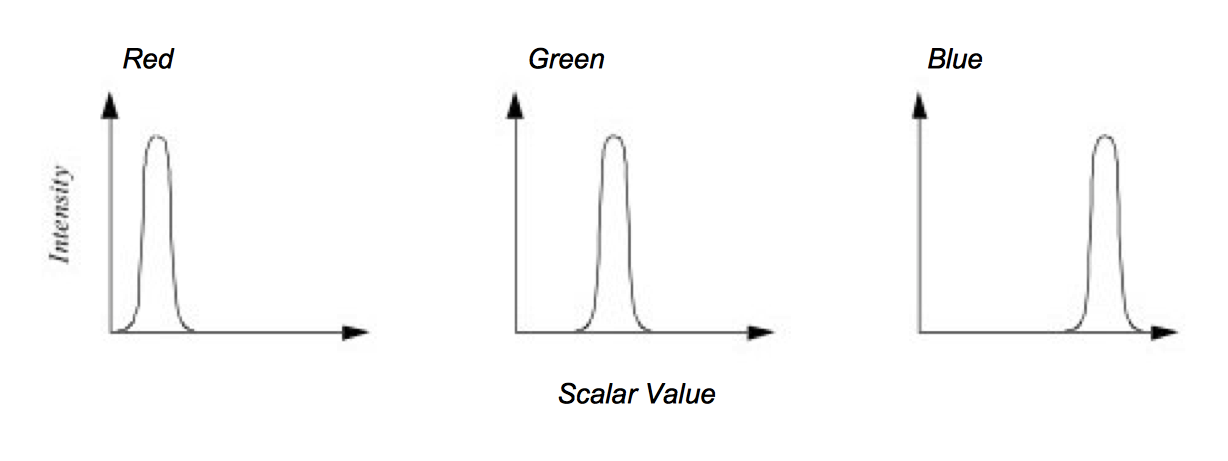
\includegraphics[width=0.8\textwidth]{Figure6-2}
	\caption{Transfer function for color components red, green and blue as a function of scalar value.}
	\label{fig:Figure6-2}
\end{figure}

\begin{figure}[!htb]
	\centering
	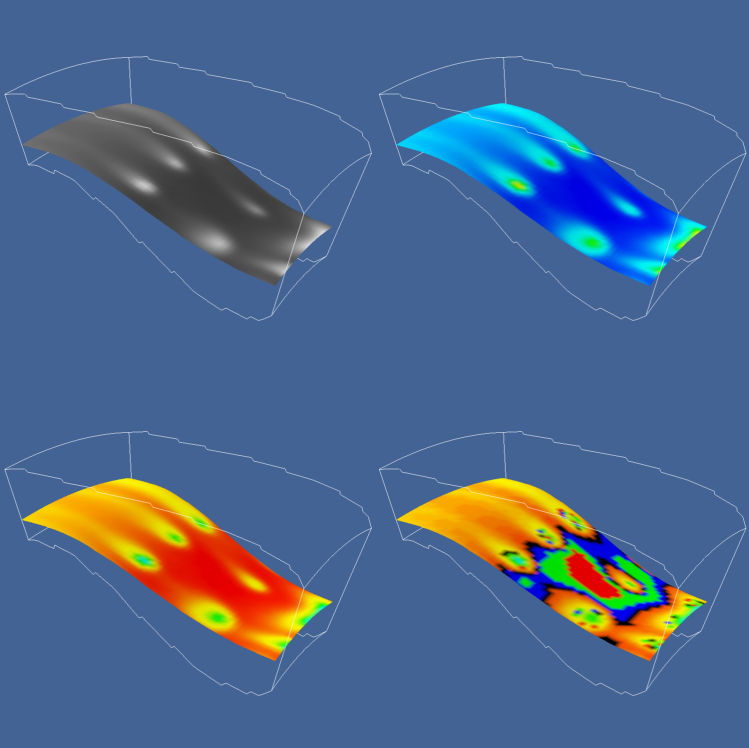
\includegraphics[width=0.8\textwidth]{Figure6-3}
	\caption{Flow density colored with different lookup tables. Top-left: grayscale; Top-right rainbow (blue to red); lower-left rainbow (red to blue); lower-right large contrast. (\href{https://lorensen.github.io/VTKExamples/site/Cxx/Rendering/Rainbow/}{Rainbow.cxx}) and (\href{https://lorensen.github.io/VTKExamples/site/Python/Rendering/Rainbow/}{Rainbow.py})}
	\label{fig:Figure6-3}
\end{figure}

\subsection{Contourning}

A natural extension to color mapping is \emph{contouring}. When we see a surface colored with data values, the eye often separates similarly colored areas into distinct regions. When we contour data, we are effectively constructing the boundary between these regions. These boundaries correspond to contour lines (2D) or surfaces (3D) of constant scalar value.

Examples of 2D contour displays include weather maps annotated with lines of constant temperature (isotherms), or topological maps drawn with lines of constant elevation. Three-dimensional contours are called \emph{isosurfaces}, and can be approximated by many polygonal primitives. Examples of isosurfaces include constant medical image intensity corresponding to body tissues such as skin, bone, or other organs. Other abstract isosurfaces such as surfaces of constant pressure or temperature in fluid flow also may be created.

\begin{figure}[!htb]
	\centering
	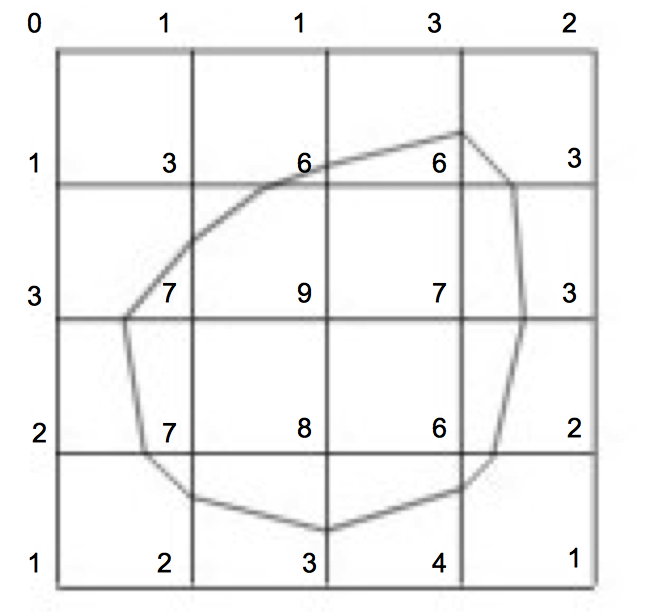
\includegraphics[width=0.8\textwidth]{Figure6-4}
	\caption{ Contouring a 2D stuctured grid with contour line value = 5.}
	\label{fig:Figure6-4}
\end{figure}

Consider the 2D structured grid shown in \ref{fig:Figure6-4}. Scalar values are shown next to the points that define the grid. Contouring always begins by selecting a scalar value, or contour value, that corresponds to the contour lines or surfaces generated. To generate the contours, some form of interpolation must be used. This is because we have scalar values at a finite set of points in the dataset, and our contour value may lie between the point values. Since the most common interpolation technique is linear, we generate points on the contour surface by linear interpolation along the edges. If an edge has scalar values 10 and 0 at its two endpoints, and if we are trying to generate a contour line of value 5, then edge interpolation computes that the contour passes through the midpoint of the edge.



\section{Bibliographic Notes}

Color mapping is a widely studied topic in imaging, computer graphics, visualization, and human factors. References \cite{Durrett87} \cite{Ware88} \cite{Rheingans92} provide samples of the available literature. You also may want to learn about the physiological and psychological effects of color on perception. The text by Wyszecki and Stiles \cite{Wyszecki82} serves as an introductory reference.

Contouring is a widely studied technique in visualization because of its importance and popularity. Early techniques were developed for 2D data \cite{Watson92}. Three-dimensional techniques were developed initially as contour connecting methods \cite{Fuchs77} --- that is, given a series of 2D contours on evenly spaced planes, connect the contours to create a closed surface. Since the introduction of marching cubes \cite{Lorensen87}, many other techniques have been implemented. (A few of these include \cite{Nielson91} \cite{Montani94} and \cite{Durst88} ). A particularly interesting reference is given by Livnat et al. \cite{Livnat96}. They show a contouring method with the addition of a preprocessing step that generates isocontours in near optimal time.

Although we barely touched the topic, the study of chaos and chaotic vibrations is a delightfully interesting topic. Besides the original paper by Lorenz \cite{Lorenz63}, the book by Moon \cite{Moon87} is a good place to start.

Two- and three-dimensional vector plots have been used by computer analysts for many years \cite{Fuller80}. Streamlines and streamribbons also have been applied to the visualization of complex flows \cite{Volpe89}. Good general references on vector visualization techniques are given in \cite{Helman90} and \cite{Richter90}.

Tensor visualization techniques are relatively few in number. Most techniques are glyph oriented \cite{Haber90} \cite{deLeeuw93}. We will see a few more techniques in Chapter 9.

Blinn \cite{Blinn82}, Bloomental \cite{Bloomenthal88} \cite{Bloomenthal97} and Wyvill \cite{Wyvill86} have been important contributors to implicit modeling. Implicit modeling is currently popular in computer graphics for modeling "soft" or "blobby" objects. These techniques are simple, powerful, and are becoming widely used for advanced computer graphics modeling.


\printbibliography


\section{Exercises}
\begin{enumerate}

\item Sketch contour cases for marching triangles. How many cases are there?

\item Sketch contour cases for marching tetrahedron. How many cases are there?

\item A common visualization technique is to animate isosurface value. The procedure is to smoothly vary isosurface value over a specified range.	
\begin{enumerate}
	\item Create an animation sequence for the quadric example ( **Figure4--1** )
	\item Create an animation sequence for the head sequence ( **Figure6-11** (b))
\end{enumerate}

\item Marching Cubes visits each cell during algorithm execution. Many of these cells do not contain the isosurface. Describe a technique to improve the performance of isosurface extraction by eliminating visits to cells not containing isosurface. ( *Hint:* use a preprocessing step to analyze data. Assume that many isosurfaces will be extracted and that the preprocessing step will not count against execution time.)

\item Scanline rasterization proceeds along horizontal spans in graphics hardware (see tion" on page54 ). Interpolation of color occurs along horizontal spans as well.
\begin{enumerate}
	\item Show how the orientation of a polygon affects interpolated color.
	\item Discuss potential problems caused by orientation dependent viewing of visualizations.
\end{enumerate}

\item Write a program to simulate beam vibration. Use the code associated with **Figure6-14** (a) as your starting point.

\item 	 Using the filters vtkStreamLine, vtkMaskPoints, and vtkGlyph3D, create a visualization consisting of oriented glyphs along a streamline.

\item Visualize the following functions.
\begin{enumerate}
	\item Scalar $S(x,y,z)=sin(xy)$ for $x,y$, between $0$ and $\pi$.
	\item The effective stress field (a scalar field) from **Figure6–21**.
	\item The vector field described in the combustor data (i.e., combq.bin and combxyz.bin ).
\end{enumerate}

\item Tensor ellipsoids are based on an ellipsoidal glyph. Describe two other glyphs that you might use.

\item Write a source object to generate a polygonal representation of a torus.

\item Design a glyph to convey airplane heading, speed, and altitude, and proximity (i.e., distance) to other planes.

\item Morphing is a process to smoothly blend images (2D) or geometry (3D) between two known images or geometry. Using an implicit modeling approach, how would you morph a torus into a cube?

\item Describe a technique to visualize vector information by animating a color map. (emph{Hint:} By choosing a map carefully, you can give the illusion of motion across a surface.)

\item Isoline contours of different values are typically shown together in one image.
\begin{enumerate}
	\item Describe the advantages and disadvantages of displaying isosurfaces simultaneously.
	\item What two graphics properties might you adjust to improve the display of multiple isosurefaces?
\end{enumerate}

\item Describe a parallel algorithm for marching cubes. Use a parallel architecture of your choice.

\item Decomposition can greatly increase the speed of an operation.
\begin{enumerate}
	\item  Prove that 3D Gaussian smoothing can be decomposed into three 1D operations.
	\item Give the complexity of the decomposed filter and the same filter implemented as a 3D convolution.
	\item Under what conditions can constant smoothing be decomposed into 1D operations.
\end{enumerate}

\end{enumerate}
